\section{Proposed KDR-CA-AEAD Architecture}
\label{sec:architecture}

\subsection{Overall System Architecture}
\label{subsec:system_arch}
The overall system architecture of KDR-CA-AEAD consists of five modular subsystems: (1) Key Derivation Engine, (2) Dynamic Rule Scheduler, (3) Candidate A-Chain State Engine, (4) CTR-PRNG Keystream Generator, and (5) Encrypt-then-MAC AEAD Integrity Engine, as illustrated in Fig. \ref{fig:system_arch}.

\begin{figure}[htbp]
\centering
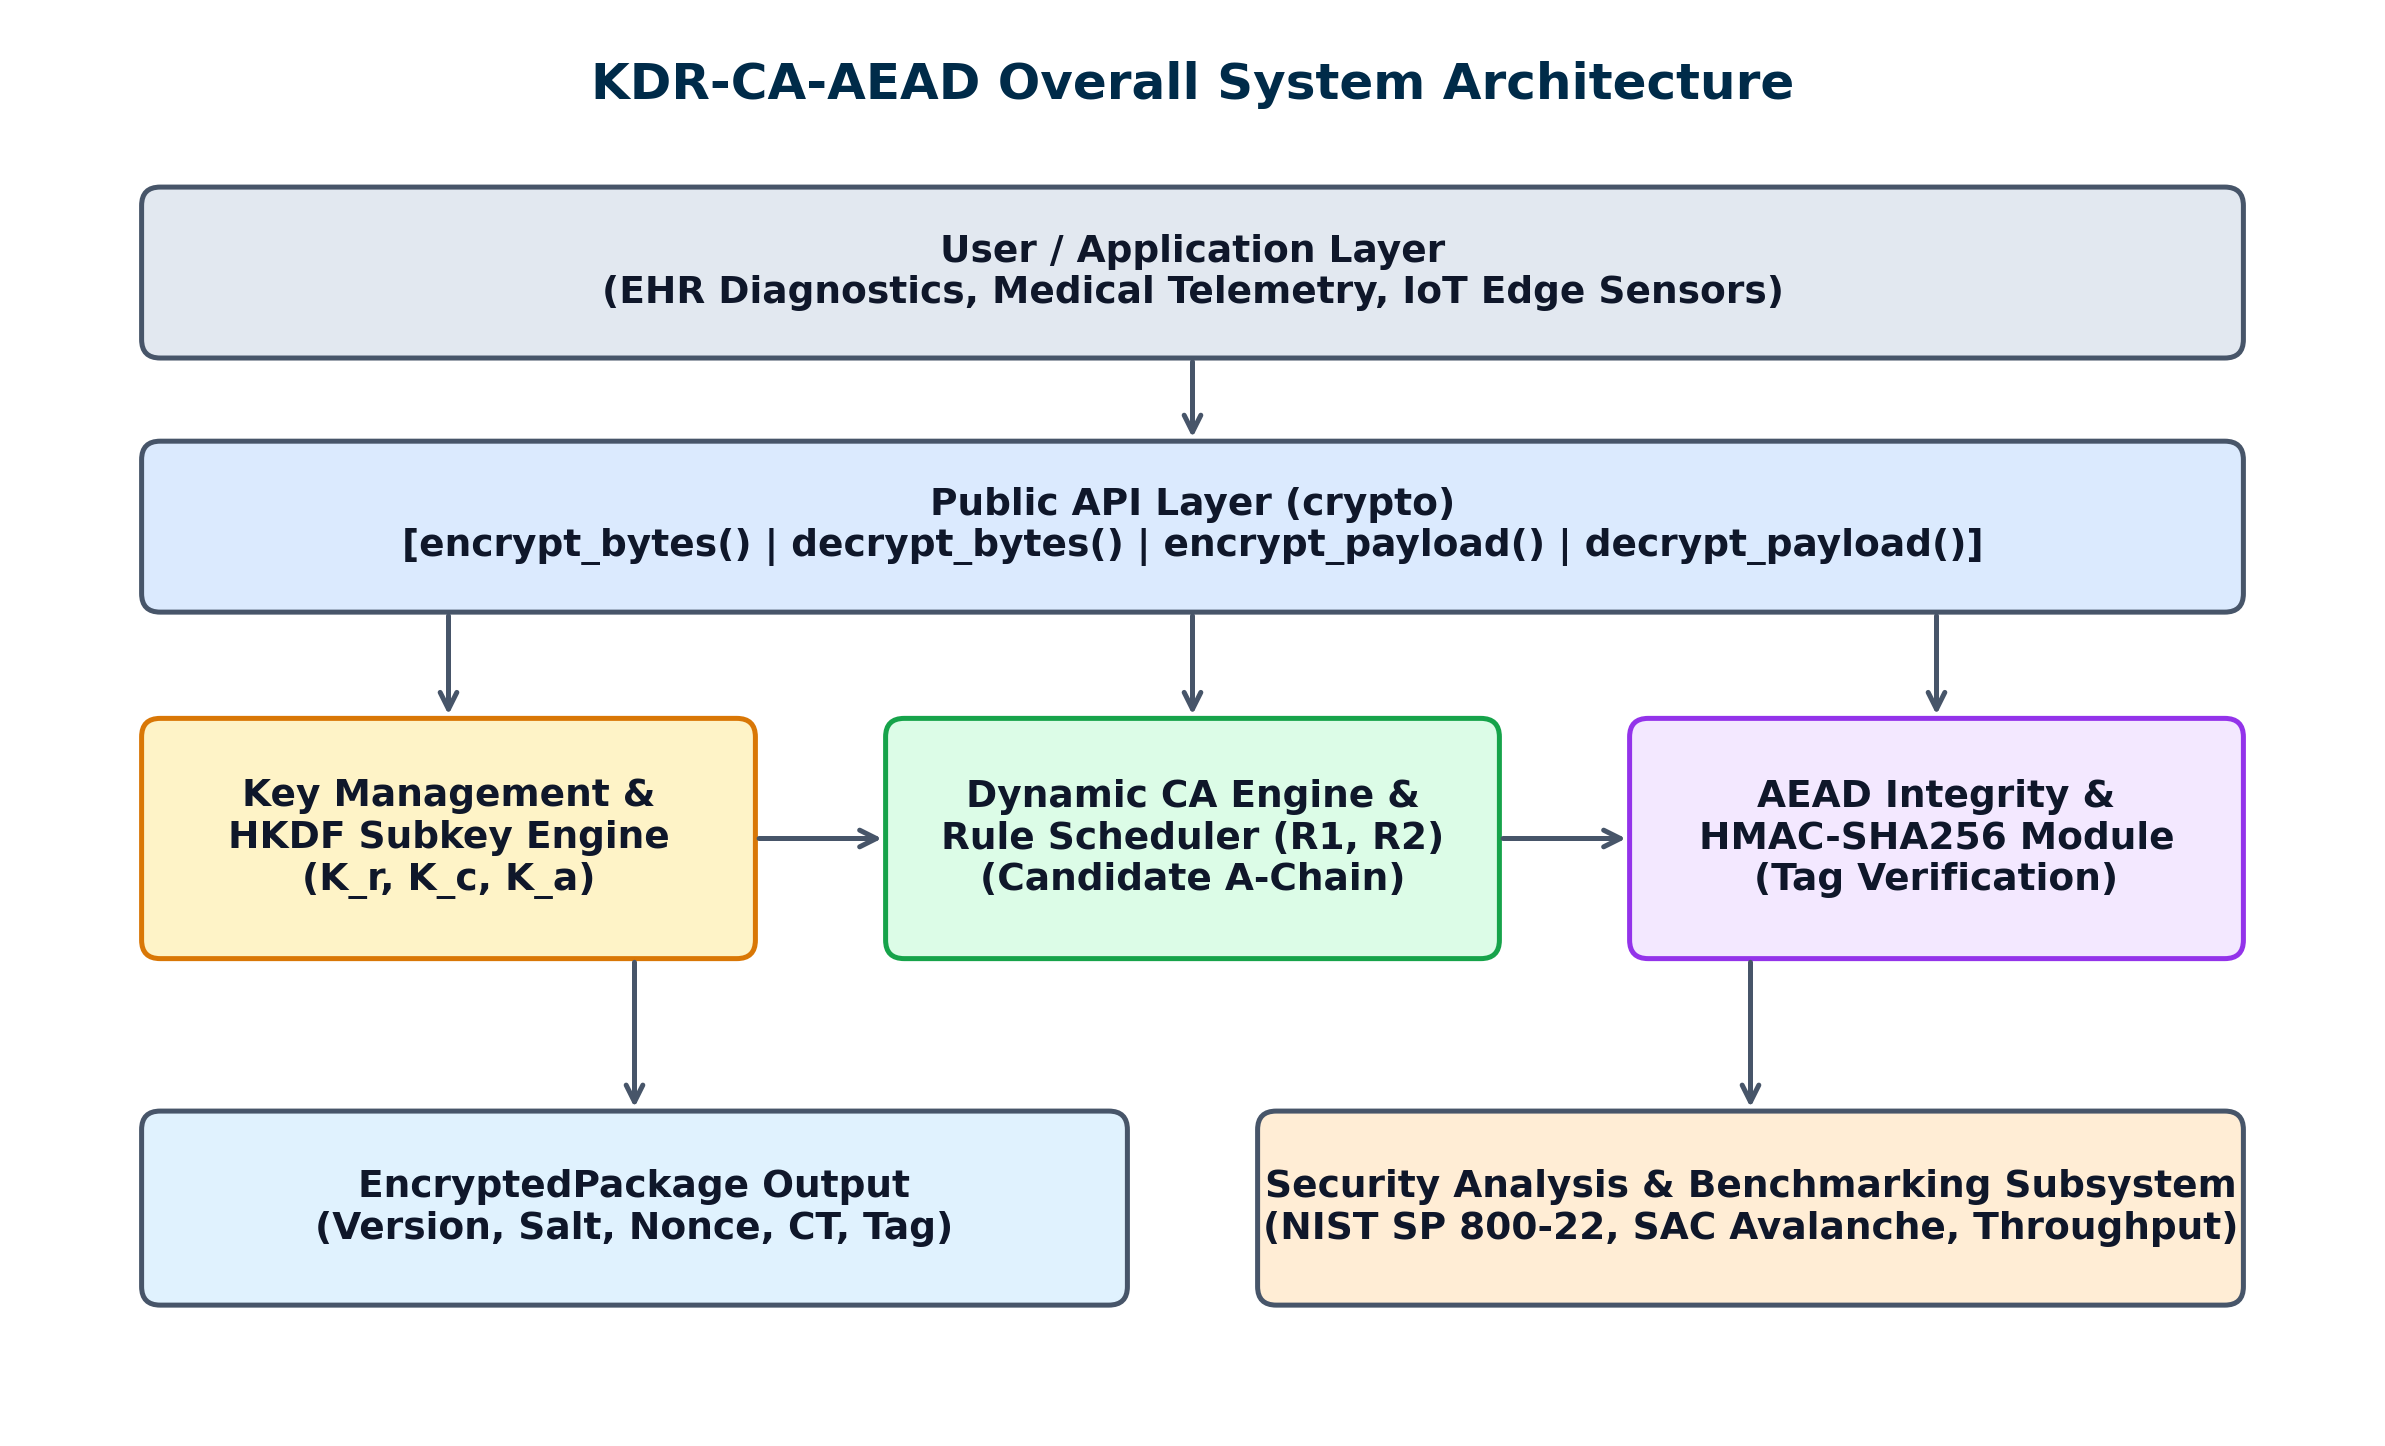
\includegraphics[width=\columnwidth]{../docs/figures/system_architecture.png}
\caption{Overall KDR-CA-AEAD 5-Layer Subsystem Architecture.}
\label{fig:system_arch}
\end{figure}

\subsection{Encryption Workflow}
\label{subsec:encryption_workflow}
The end-to-end encryption workflow is illustrated in Fig. \ref{fig:encryption_flow} and summarized in Algorithm \ref{alg:encryption}.

\begin{figure}[htbp]
\centering
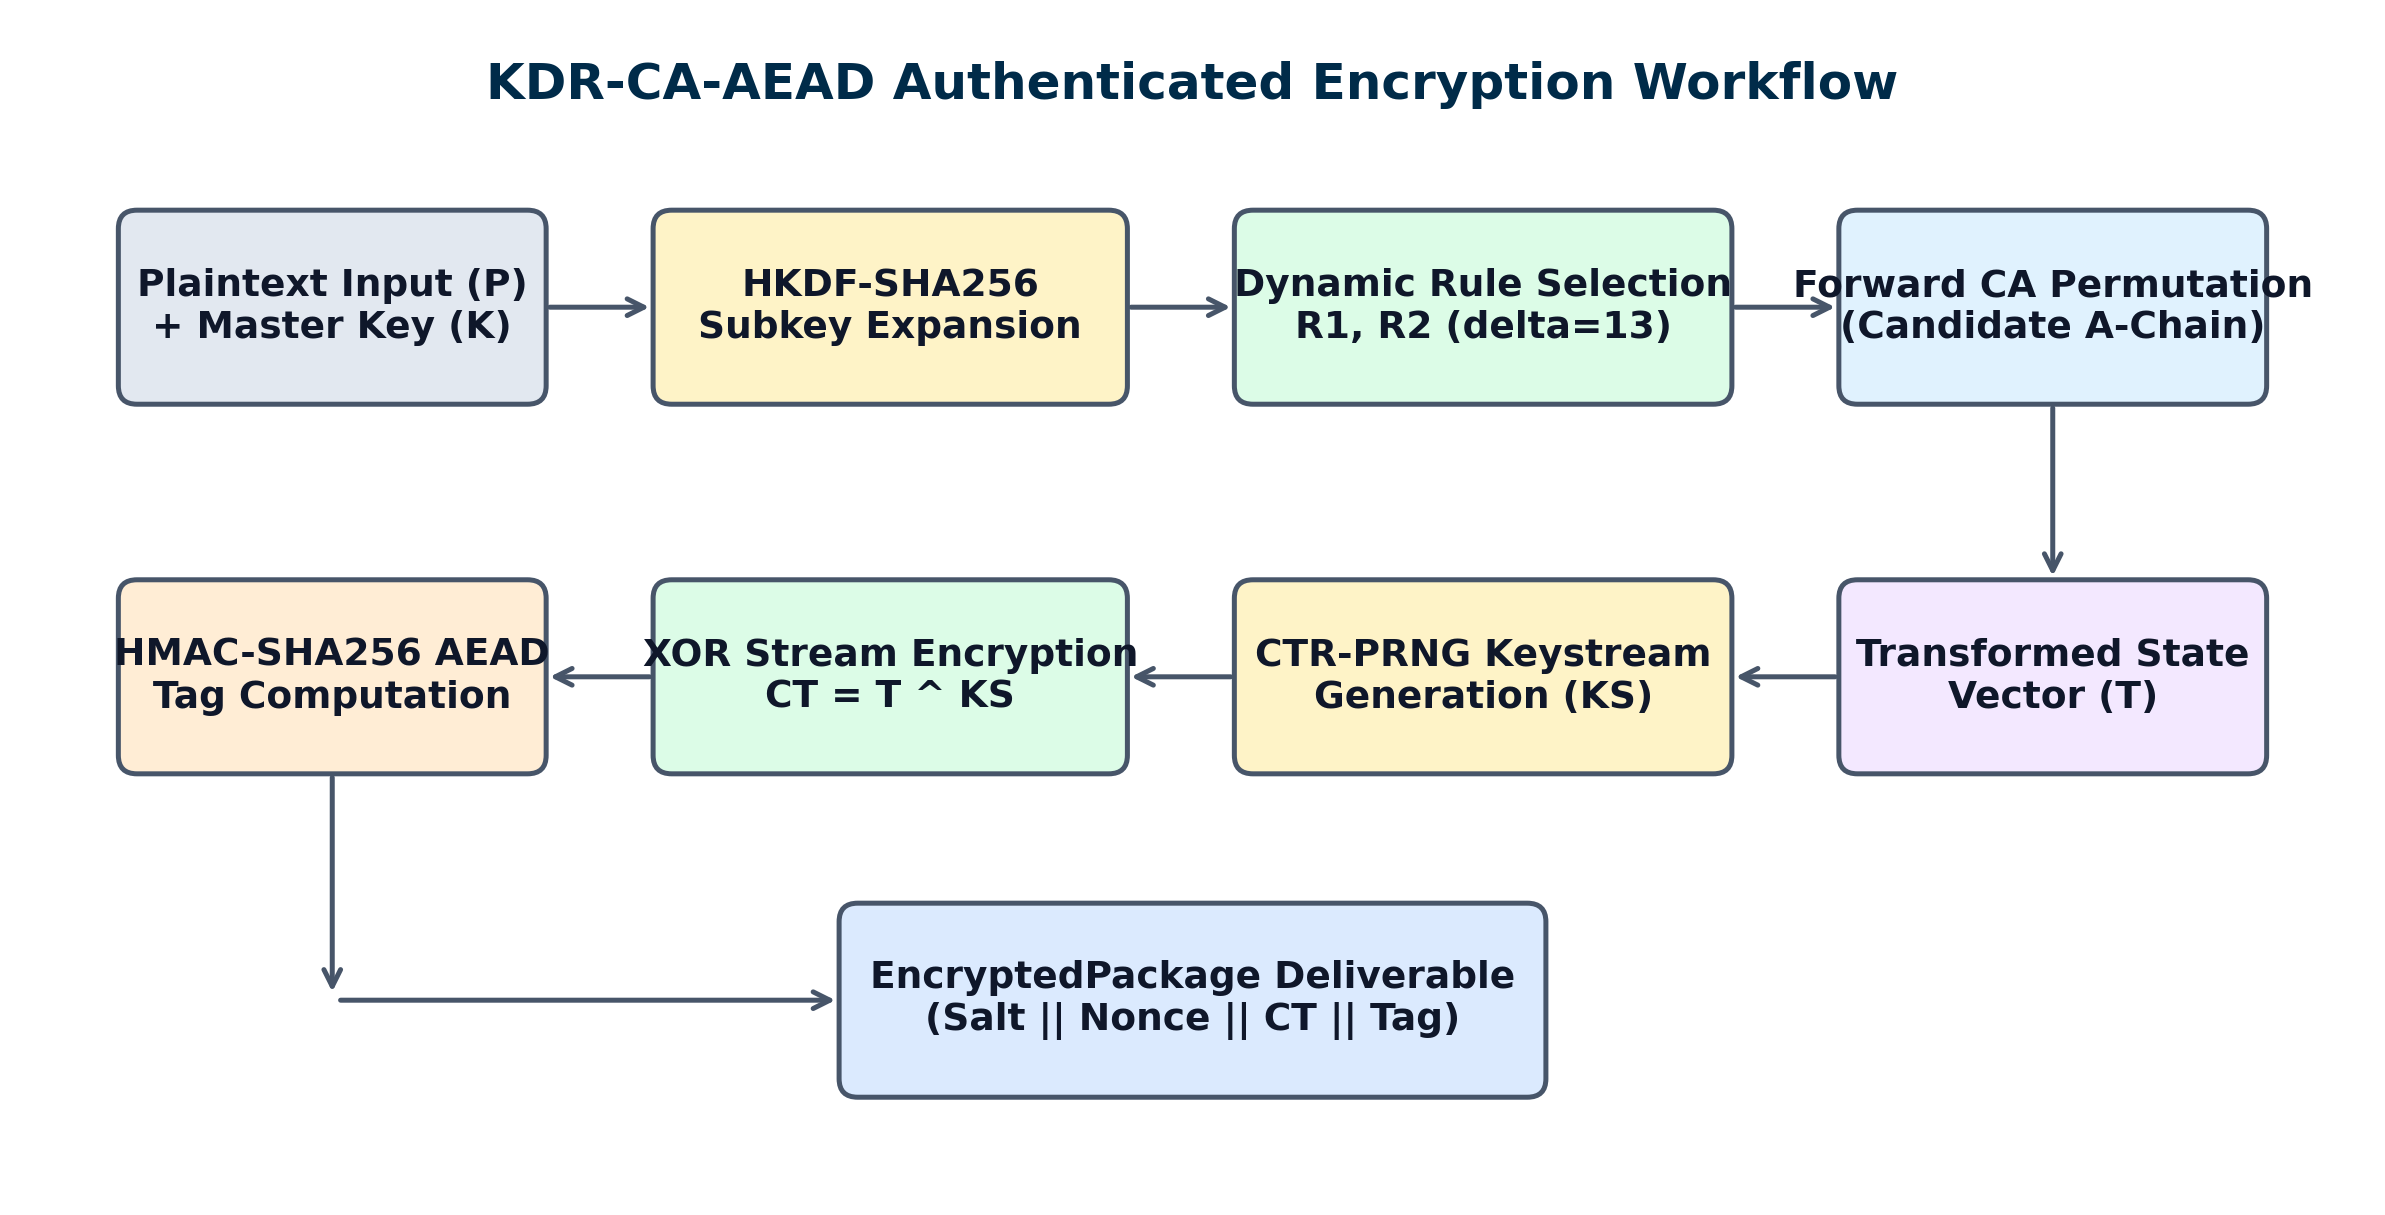
\includegraphics[width=\columnwidth]{../docs/figures/encryption_workflow.png}
\caption{KDR-CA-AEAD Authenticated Encryption Workflow.}
\label{fig:encryption_flow}
\end{figure}

\begin{algorithm}[htbp]
\caption{KDR-CA-AEAD Authenticated Encryption Pipeline}
\label{alg:encryption}
\begin{algorithmic}[1]
\REQUIRE Plaintext $P$, Master Key $K$, Optional Associated Data $AD$, Salt $S$, Nonce $N$
\ENSURE EncryptedPackage $(V, S, N, CT, \text{Tag})$
\IF{$S$ is \textbf{null}}
    \STATE $S \leftarrow \text{CSPRNG\_Generate}(16)$
\ENDIF
\IF{$N$ is \textbf{null}}
    \STATE $N \leftarrow \text{CSPRNG\_Generate}(12)$
\ENDIF
\STATE $(K_r, K_c, K_a, R) \leftarrow \text{HKDF\_SubKey\_Derivation}(K, S, N)$
\STATE $T \leftarrow \text{Candidate\_A\_Chain\_Forward}(P, R)$
\STATE $KS \leftarrow \text{HMAC\_SHA256\_CTR\_Keystream}(K_c, N, \text{Length}(T))$
\STATE $CT \leftarrow T \oplus KS$
\STATE $\text{Tag} \leftarrow \text{HMAC\_SHA256}(K_a, N \,\|\, S \,\|\, AD \,\|\, CT)$
\RETURN $\text{EncryptedPackage}(V=\text{"KDR-CA-AEAD-v1"}, S, N, CT, \text{Tag})$
\end{algorithmic}
\end{algorithm}

\subsection{Decryption Workflow}
\label{subsec:decryption_workflow}
The end-to-end decryption workflow is illustrated in Fig. \ref{fig:decryption_flow} and summarized in Algorithm \ref{alg:decryption}.

\begin{figure}[htbp]
\centering
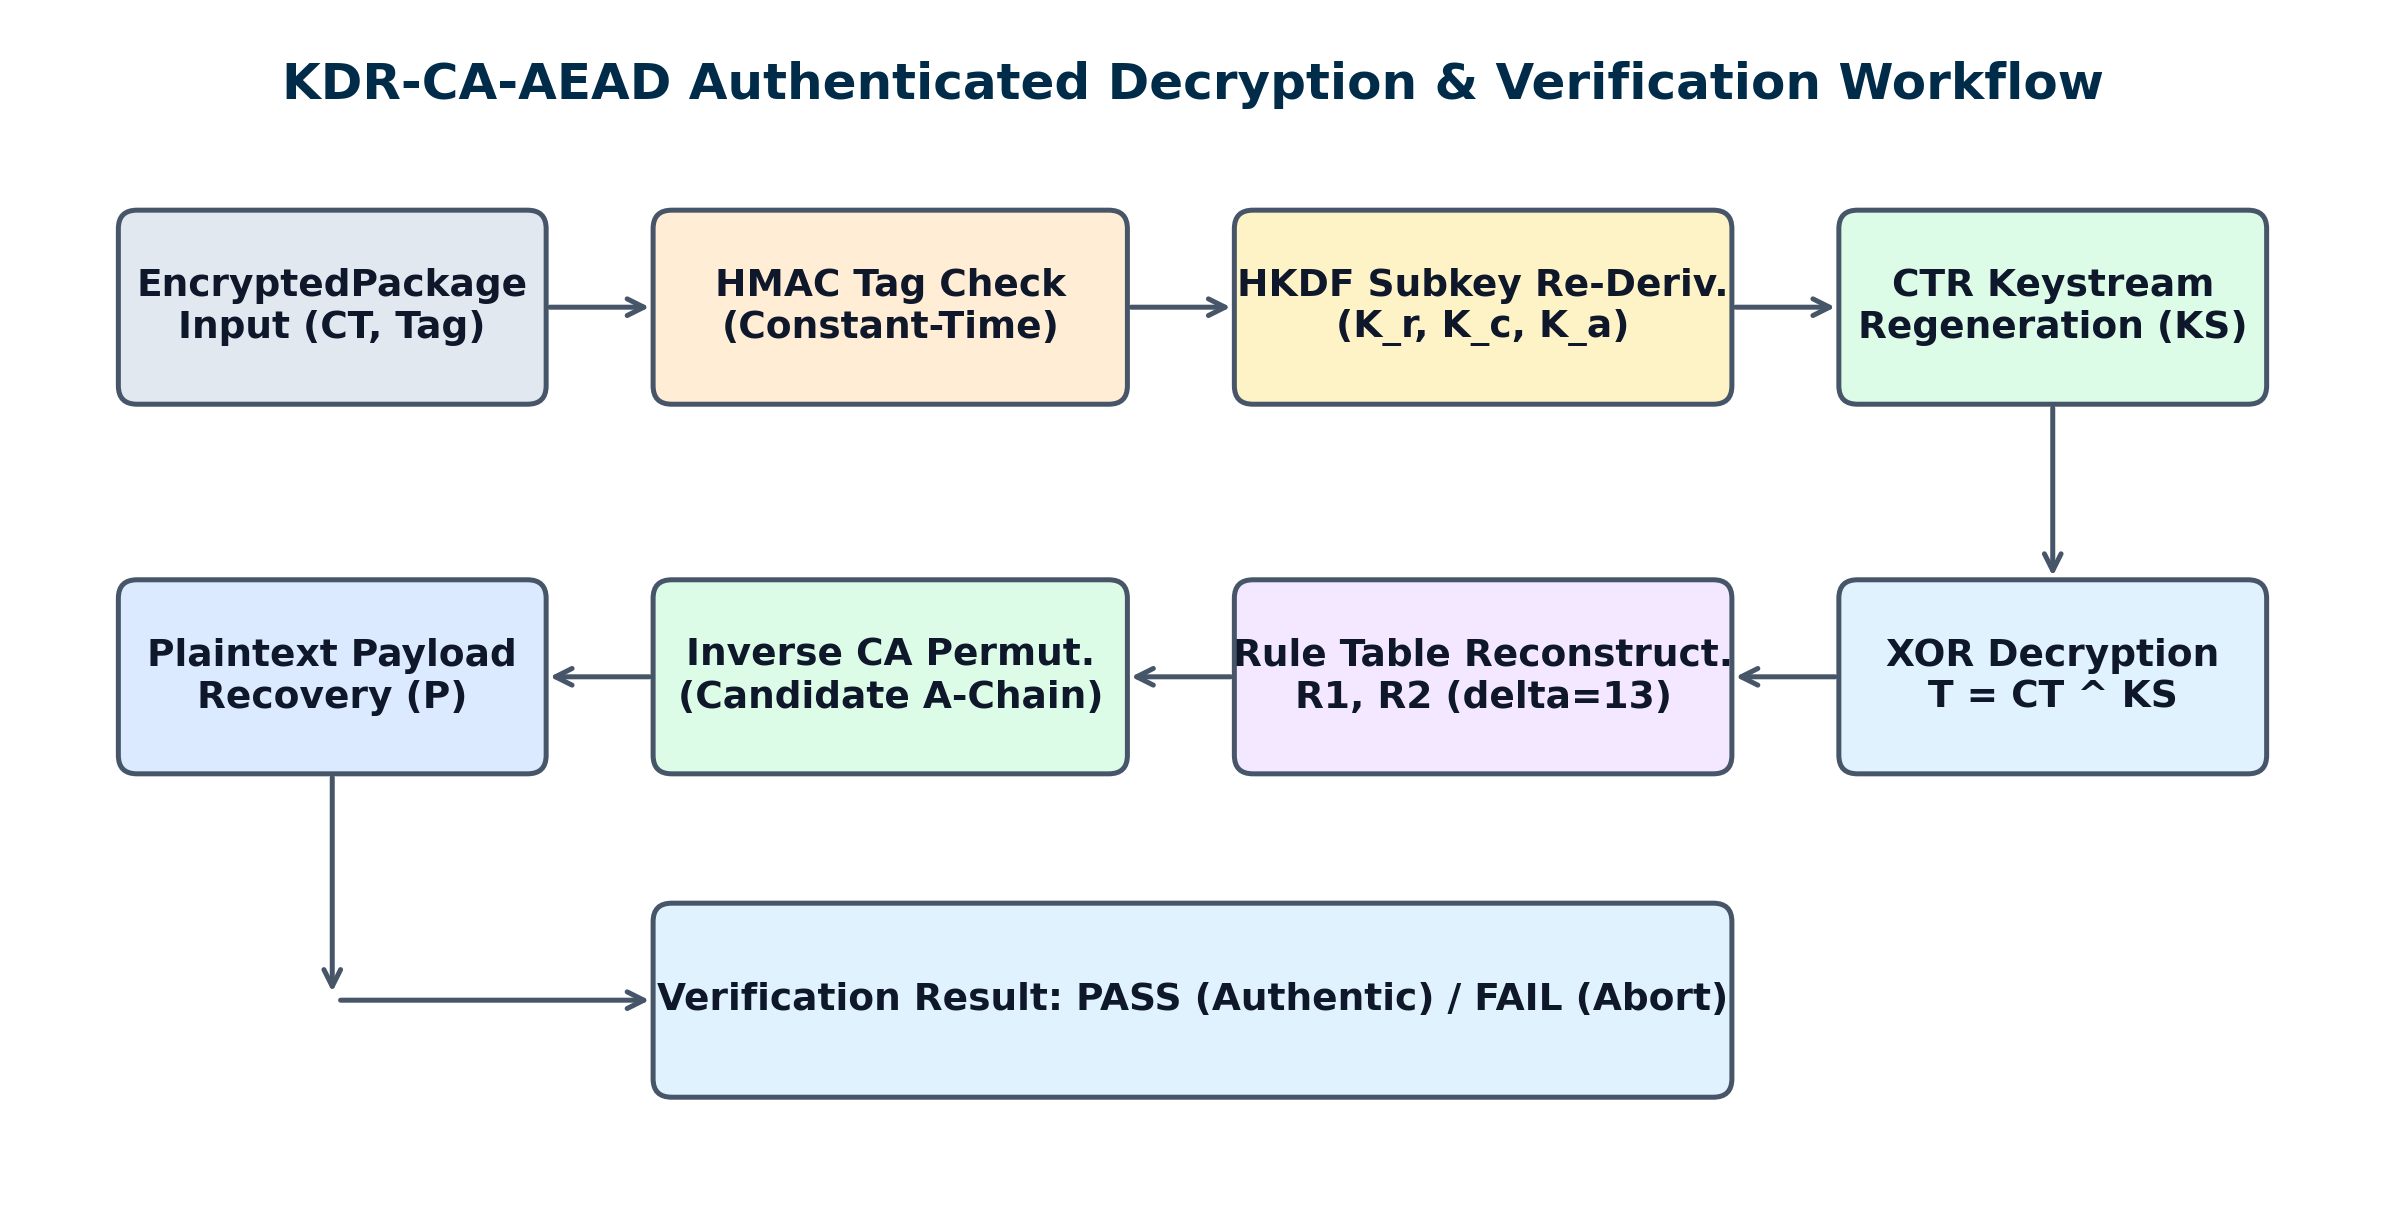
\includegraphics[width=\columnwidth]{../docs/figures/decryption_workflow.png}
\caption{KDR-CA-AEAD Authenticated Decryption \& Verification Workflow.}
\label{fig:decryption_flow}
\end{figure}

\begin{algorithm}[htbp]
\caption{KDR-CA-AEAD Authenticated Decryption Pipeline}
\label{alg:decryption}
\begin{algorithmic}[1]
\REQUIRE EncryptedPackage $(V, S, N, CT, \text{Tag})$, Master Key $K$, Optional $AD$
\ENSURE Plaintext $P$ (or AuthenticationError)
\STATE $(K_r, K_c, K_a, R) \leftarrow \text{HKDF\_SubKey\_Derivation}(K, S, N)$
\STATE $\text{ExpectedTag} \leftarrow \text{HMAC\_SHA256}(K_a, N \,\|\, S \,\|\, AD \,\|\, CT)$
\IF{$\text{ConstantTimeCompare}(\text{Tag}, \text{ExpectedTag}) = \textbf{false}$}
    \STATE \textbf{raise} $\text{AuthenticationError("AEAD Tag Mismatch!")}$
\ENDIF
\STATE $KS \leftarrow \text{HMAC\_SHA256\_CTR\_Keystream}(K_c, N, \text{Length}(CT))$
\STATE $T \leftarrow CT \oplus KS$
\STATE $P \leftarrow \text{Candidate\_A\_Chain\_Inverse}(T, R)$
\RETURN $P$
\end{algorithmic}
\end{algorithm}

\subsection{Dynamic Cellular Automata Engine & Key Schedule}
\label{subsec:dynamic_ca_engine_fig}
The Candidate A-Chain Dynamic CA non-linear permutation engine is detailed in Fig. \ref{fig:dynamic_ca_engine}. The HKDF-SHA256 key schedule architecture is depicted in Fig. \ref{fig:key_schedule}. The Encrypt-then-MAC authentication pipeline is shown in Fig. \ref{fig:auth_enc_pipeline}.

\begin{figure}[htbp]
\centering
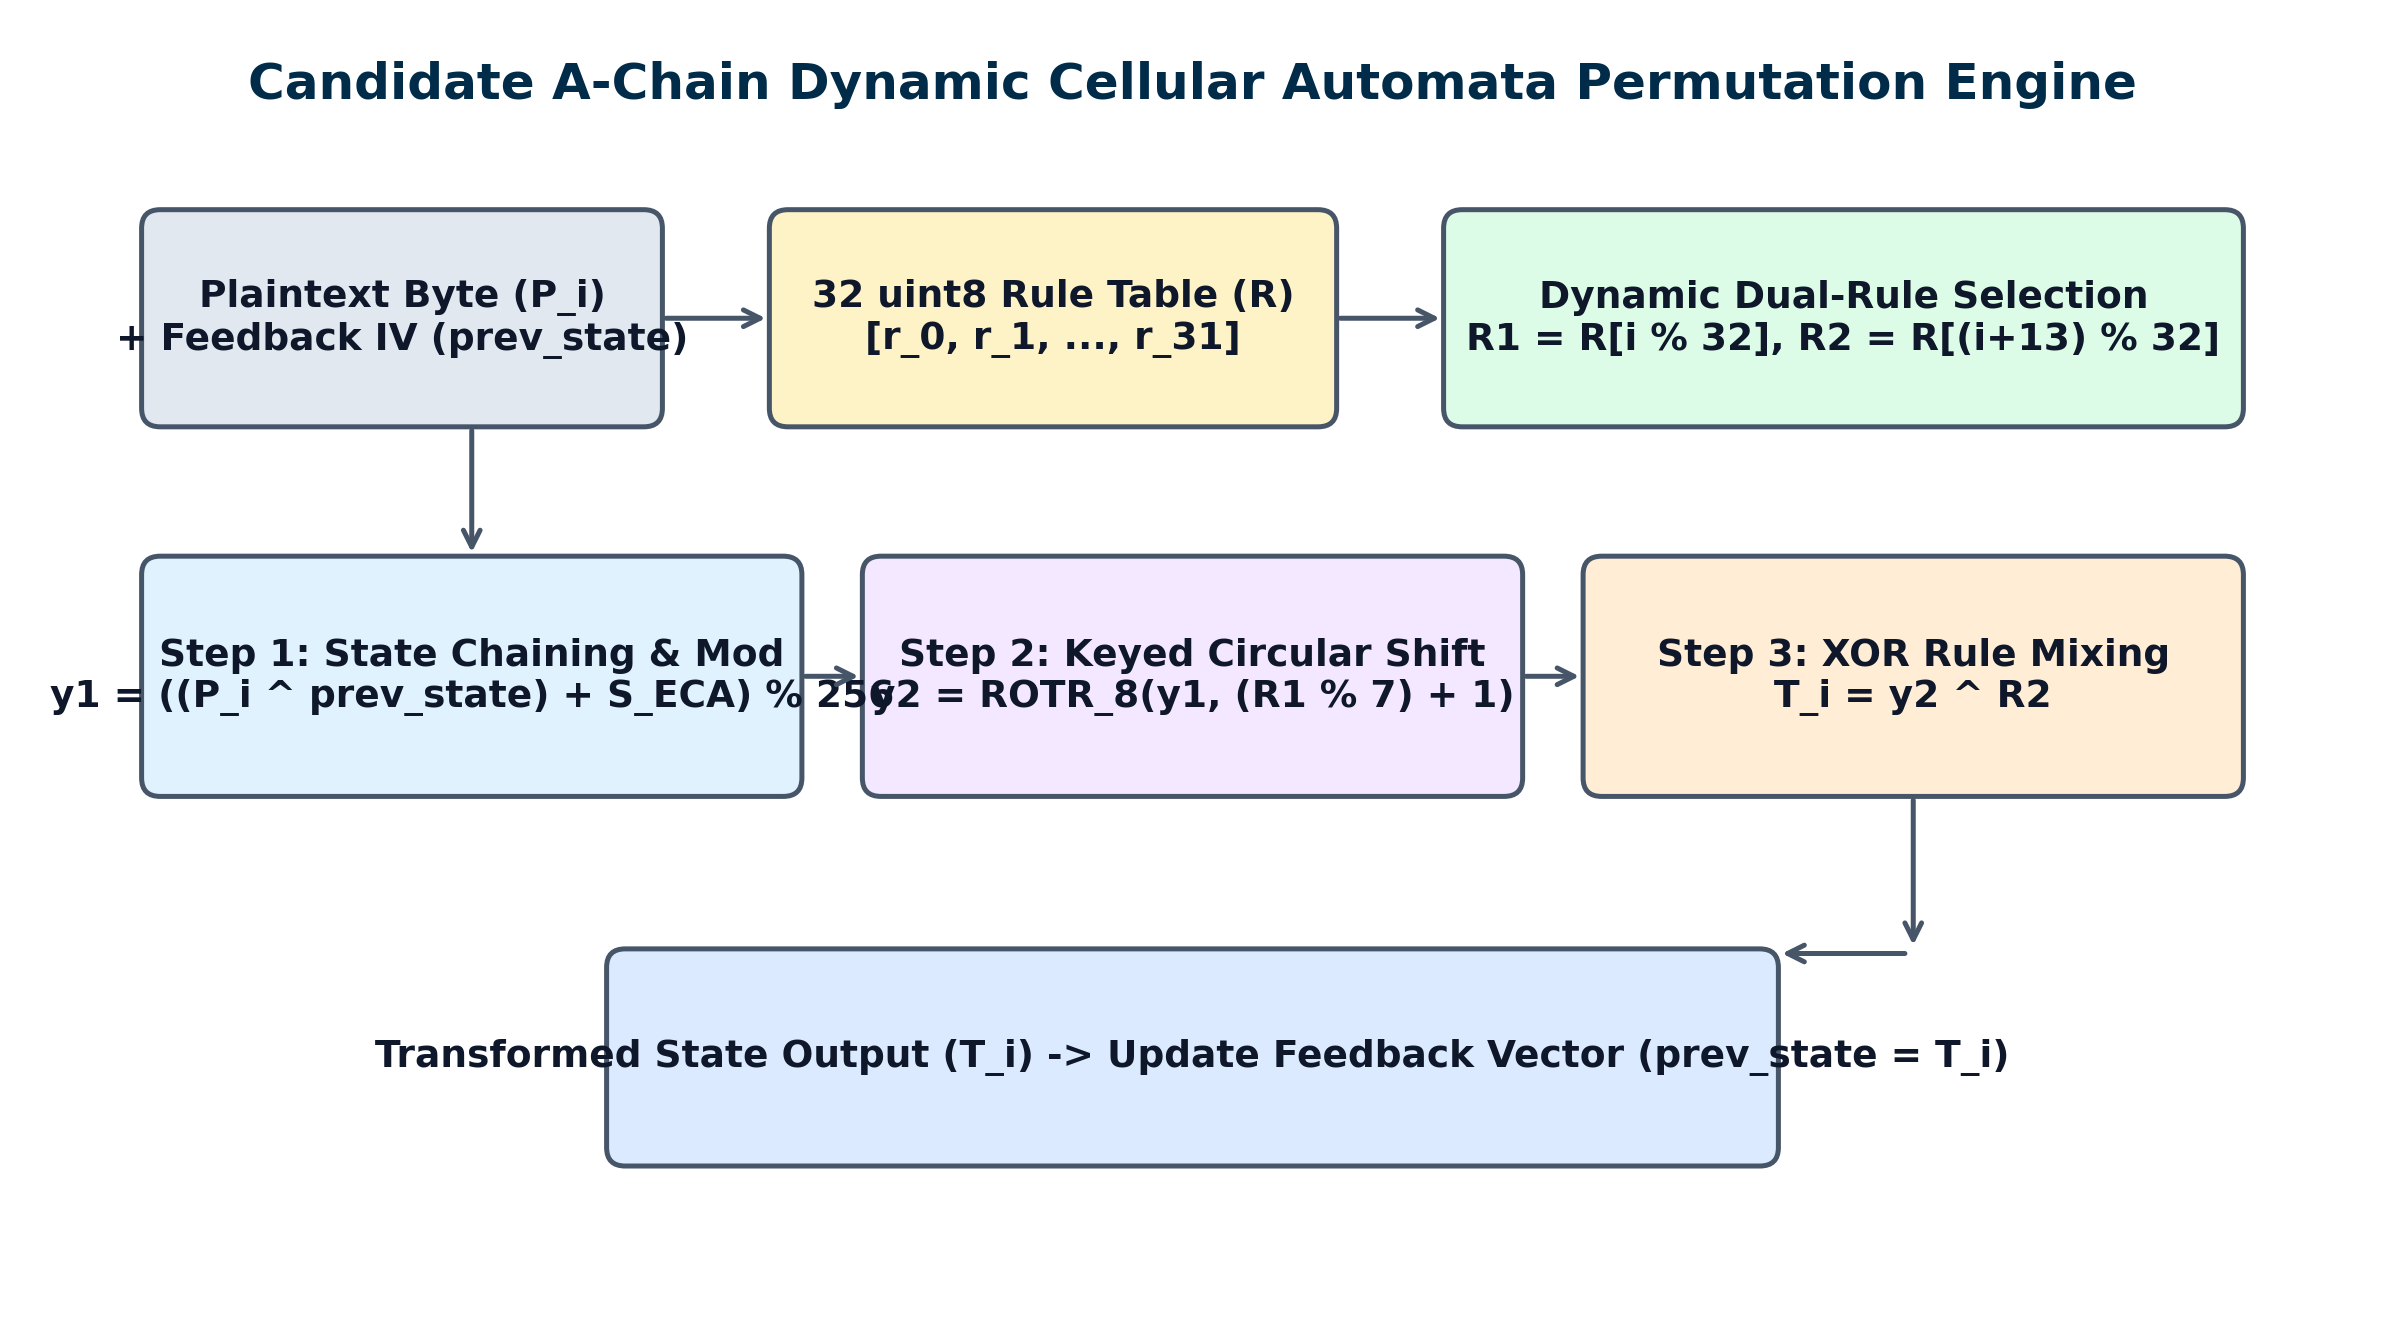
\includegraphics[width=\columnwidth]{../docs/figures/dynamic_ca_engine.png}
\caption{Candidate A-Chain Dynamic Cellular Automata Permutation Engine.}
\label{fig:dynamic_ca_engine}
\end{figure}

\begin{figure}[htbp]
\centering
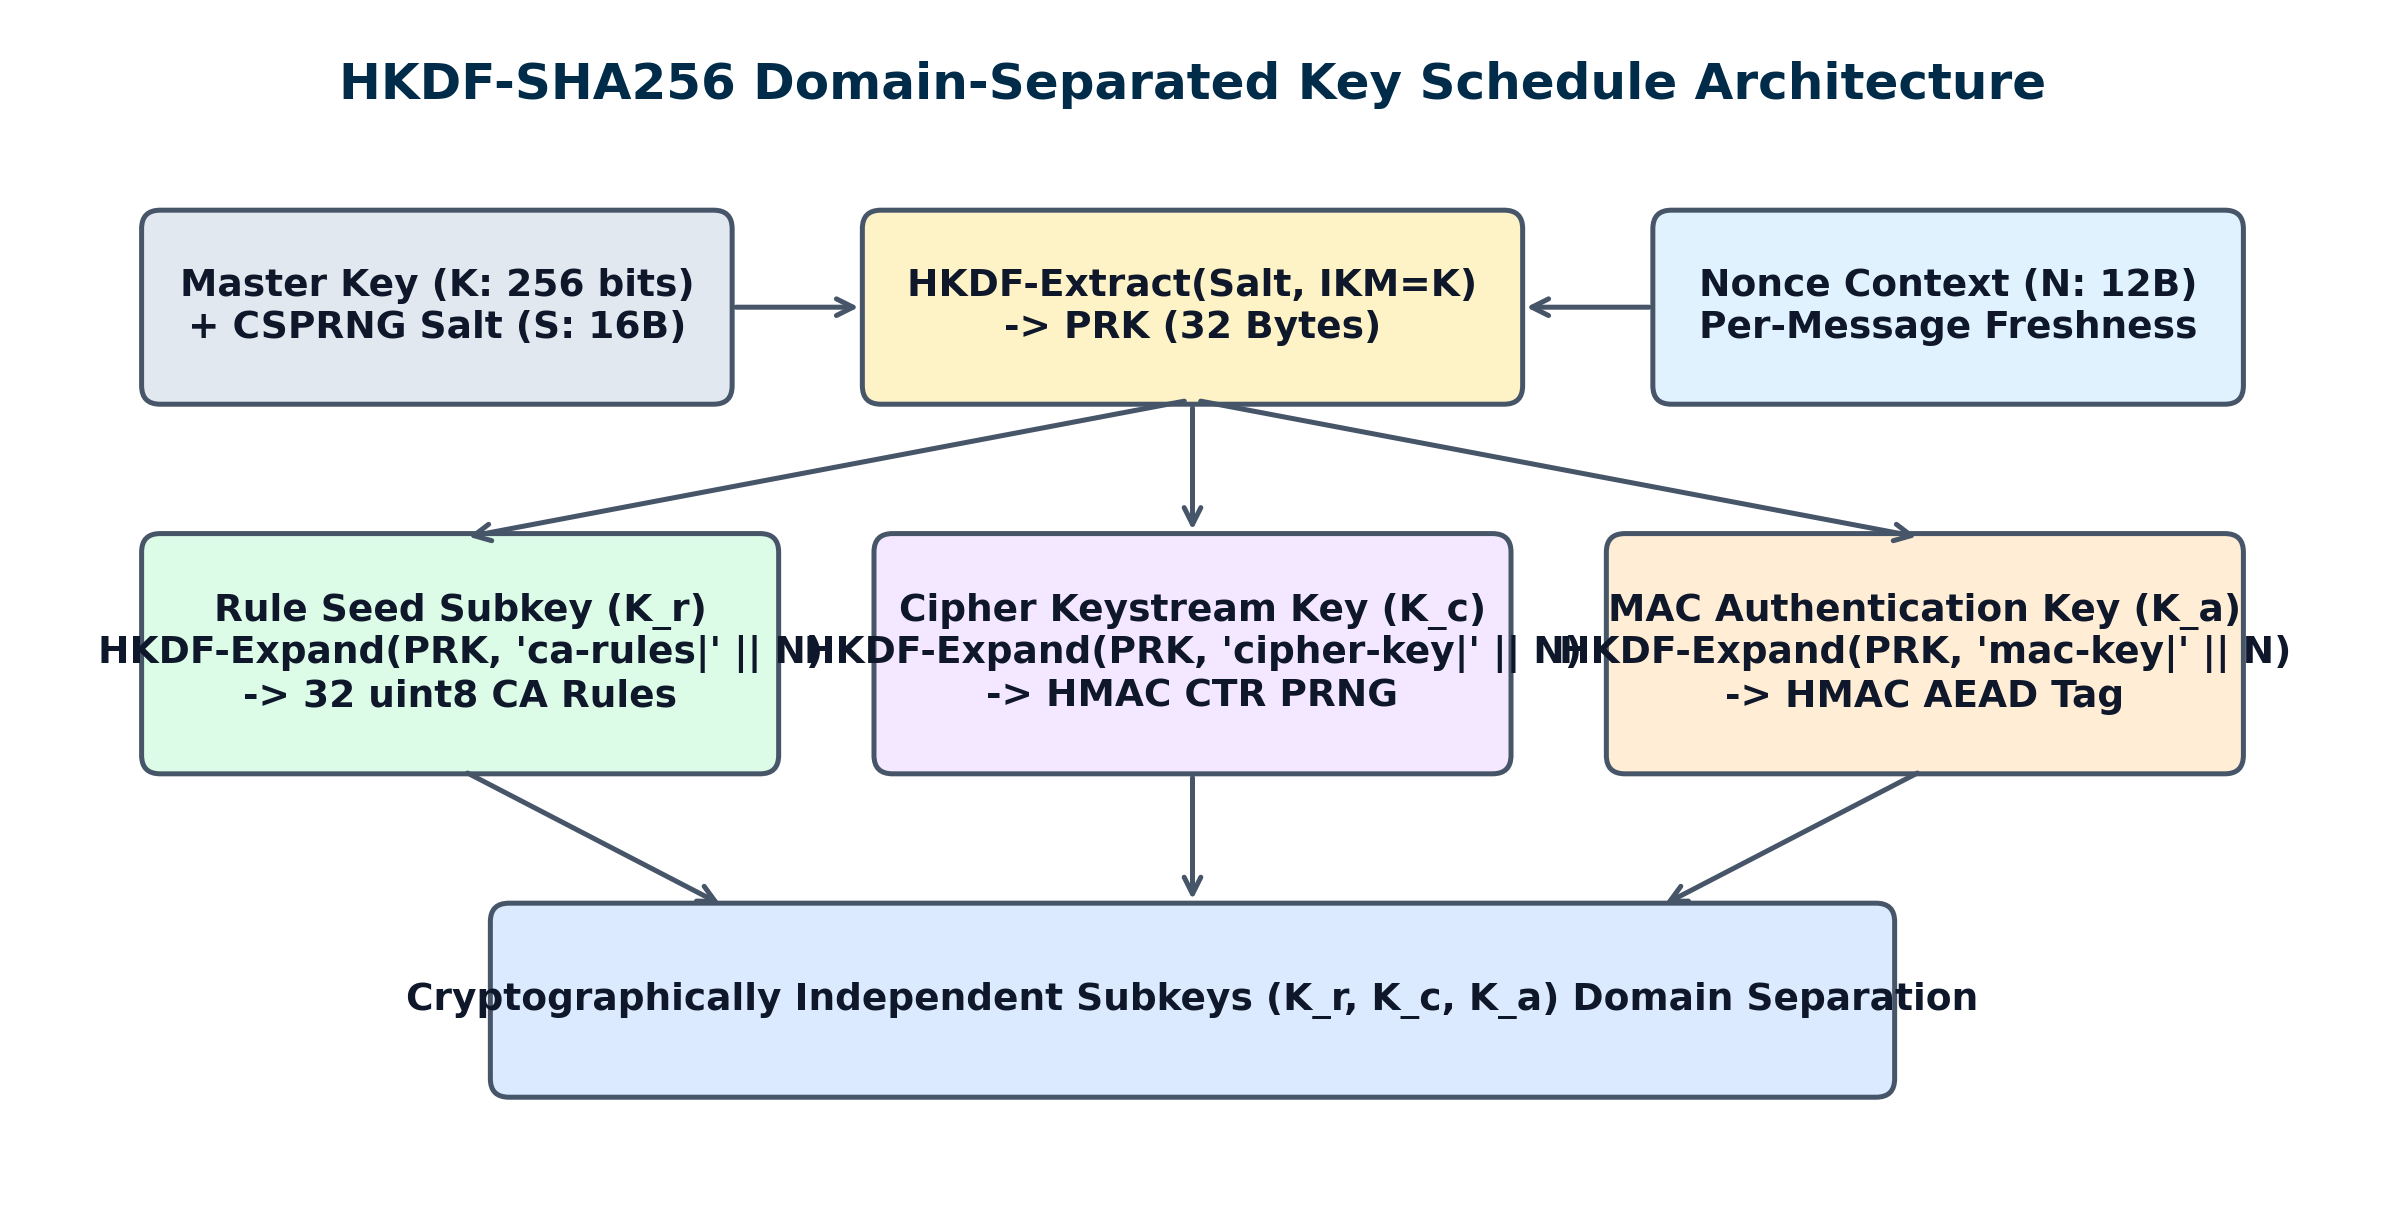
\includegraphics[width=\columnwidth]{../docs/figures/key_schedule.png}
\caption{HKDF-SHA256 Domain-Separated Key Schedule Architecture.}
\label{fig:key_schedule}
\end{figure}

\begin{figure}[htbp]
\centering
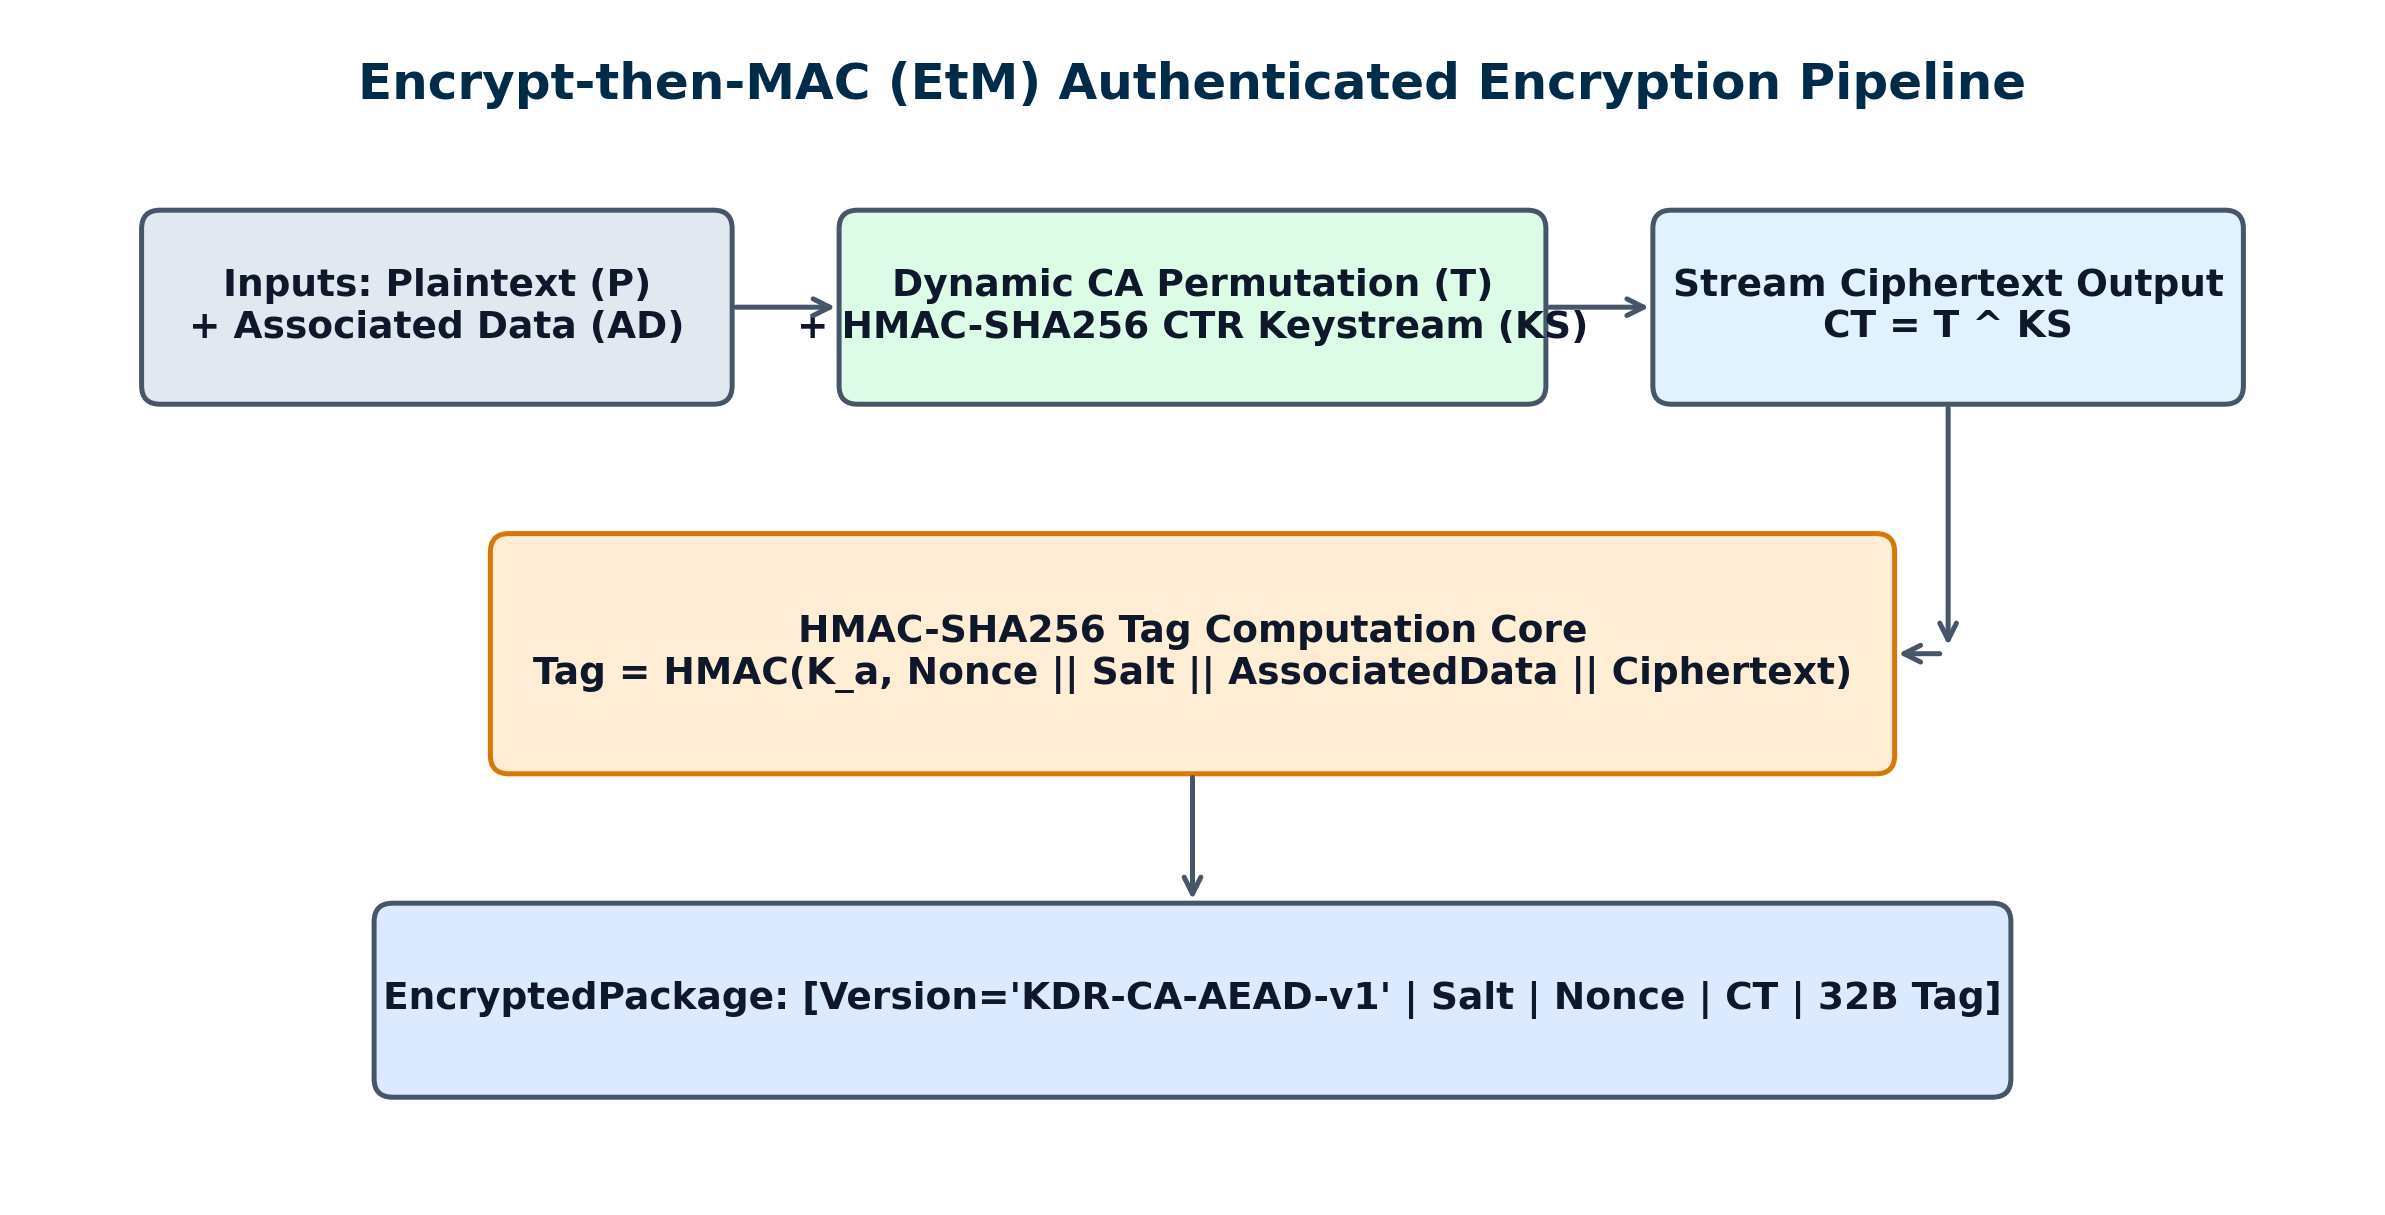
\includegraphics[width=\columnwidth]{../docs/figures/authenticated_encryption_pipeline.png}
\caption{Encrypt-then-MAC (EtM) Authenticated Encryption Core Pipeline.}
\label{fig:auth_enc_pipeline}
\end{figure}

\subsection{Keystream CTR-PRNG Generation}
\label{subsec:ctr_keystream}
The keystream generator produces pseudo-random bytes $KS$ of length $M$ using HMAC-SHA256 in counter mode. For block counter index $j \ge 0$:
\begin{equation}
\text{block}_j = \text{HMAC-SHA256}(K_c, N \,\|\, \text{to\_bytes}_4(j))
\end{equation}
Concatenating blocks $\text{block}_0 \,\|\, \text{block}_1 \,\|\, \dots$ and truncating to $M$ bytes yields the keystream $KS$. Because $K_c$ is derived per-session with CSPRNG nonce $N$, keystream reuse across distinct encryptions is impossible.
